\chapter{实践部分}
\section{TensorFlow例子}
\subsection{卷积神经网络处理序列数据}
数据集\href{https://archive.ics.uci.edu/ml/machine-learning-databases/00240/UCI%20HAR%20Dataset.names}{(HAR Dataset)}介绍:该数据集来自于智能手机获取的人活动数据,追踪人的活动状态,总共有如下六种情况:
\begin{itemize}
\item 行走
\item 上楼梯
\item 下楼梯
\item 坐立
\item 站立
\item 平躺
\end{itemize}
数据有来自加速度计和陀螺仪的数据,数据集分为测试集和训练集,训练集数据有7352个数据,数据包括如下:
\begin{itemize}
	\item body\_acc:从总的加速度中减去重力获得的加速度信号(128个值组成)
	\item body\_gyro:陀螺仪获得角速度(128个值组成)
	\item total\_acc:总的加速度(128个值组成)
\end{itemize}每个数据有128个特征。测试集有2947个数据

卷积神经网络架构如下:
\begin{figure}[H]
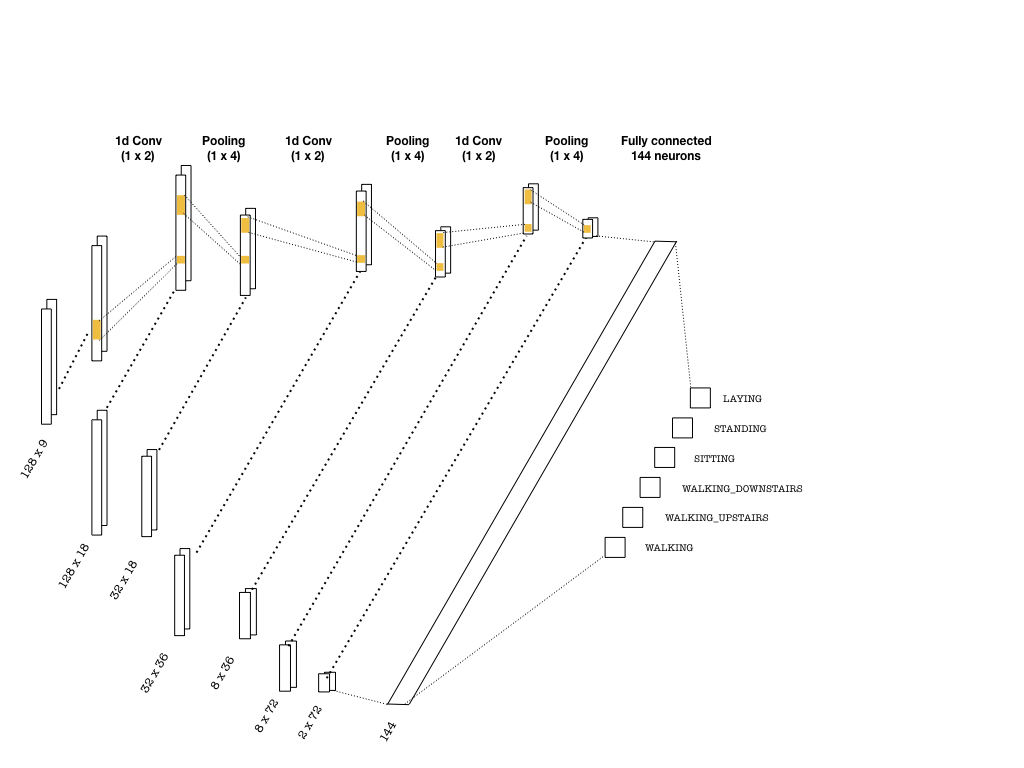
\includegraphics[scale=0.5]{HAR_cnn.png}
\caption{CNN处理HAR数据的架构}
\end{figure}
数据预处理模块:
\lstinputlisting[language=Python]{./code/har/utilities.py}
神经网络实现模块:
\lstinputlisting[language=Python]{./code/har/cnn_har.py}
